% !TeX spellcheck = sk_SK-Slovak
\chapter{Získavanie dát}

V tejto kapitole si povieme niečo o jednotlivých získavaných dátach o problémoch ktorý sa pri ich získavaní vyskytli a ako sme tieto problémy riešili.

\section{Osobné údaje pacienta a obdobie hospitalizácie}

Ako prvé boli získavané dáta nachádzajúce sa v hlavičke dokumentu konkrétne išlo o meno pacienta, jeho rodné číslo dátumy prijatia a prepustenia. Zároveň sa v tejto časti dopočítavali 2 hodnoty a to vek pacienta a dĺžka hospitalizácie.

Hlavička má výzor tabuľky s dvomi riadkami a štyrmi alebo piatimi stĺpcami v závislosti od toho či bol pacient počas hospitalizácie preložený z infekčného oddelenia na jednotku intenzívnej starostlivosti (JIS) respektíve na iného oddelenie alebo nie. Konkrétne v prípade ak pacient nebol preložený na iné oddelenie počas hospitalizácie hlavička vyzerá ako na obrázku \ref{obr:hlav_a} a v prípade, že preložený bol tak vyzerá takto ako na obrázku \ref{obr:hlav_b}.  

\begin{figure}
	%vlozenie samotneho obrazku vycentrovaneho a vhodnej velkosti
	%obrazok je v subore images/cervik.png
	\centerline{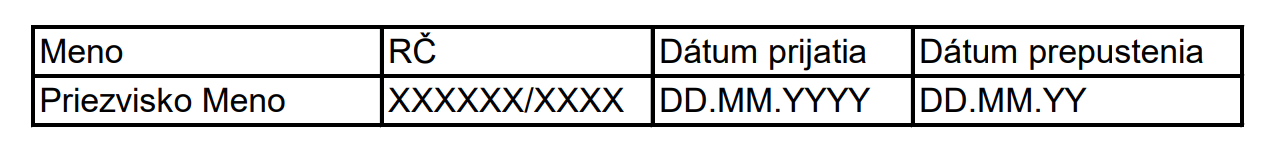
\includegraphics[width=0.9\textwidth]{images/hlavicka_a}}
	%popis obrazku
	\caption[Hlavička a)]{Výzor hlavička pacienta ktorý nebol preložený na JIS}
	%id obrazku, pomocou ktoreho sa budeme na obrazok odvolavat
	\label{obr:hlav_a}
\end{figure}

\begin{figure}
	%vlozenie samotneho obrazku vycentrovaneho a vhodnej velkosti
	%obrazok je v subore images/cervik.png
	\centerline{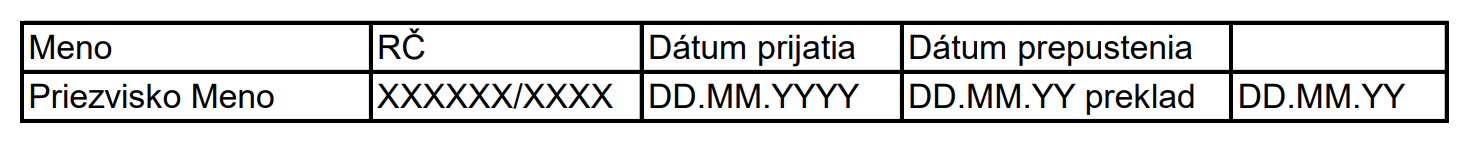
\includegraphics[width=1\textwidth]{images/hlavicka_b}}
	%popis obrazku
	\caption[Hlavička b)]{Výzor hlavička pacienta ktorý bol preložený na JIS}
	%id obrazku, pomocou ktoreho sa budeme na obrazok odvolavat
	\label{obr:hlav_b}
\end{figure}

Softvér z tejto tabuľky vyberie hodnoty z druhého riadka pričom v prípade, že v štvrtom stĺpci nájde informáciu o preklade na iné oddelenie tak dátum v tomto stĺpci ignoruje a za dátum prepustenia považuje dátum v piatom stĺpci.

Dátumy prijatia a prepustenia sú následne pre-typované do podoby časovej značky čím sa zároveň skontroluje platnosť dátumu (či taký dátum môže existovať) v prípade, že pri niektorom z dátumov vyskytne problém je táto informácia zapísaná do logovacieho súboru. V prípade, že sú obe dátumy v poriadku je následne spravený ich rozdiel čím sa vypočíta dĺžka hospitalizácie, čiže počet dní medzi prijatím a prepustením pričom tento výsledok nám dáva ďalšiu kontrolu dátumov keďže očakávame, že dĺžka hospitalizácie je kladné číslo avšak nepredpokladáme, že to číslo bude veľmi veľké, konkrétne pri testovaní sa ukázalo, že priemerná dĺžka hospitalizácie je približne 12 dní pričom štandardná odchýlka je približne 9 dní avšak občas sa objavia aj prípady ktorých dĺžka hospitalizácie je cez 50 dní pričom nenastal žiaden preklep pri zapisovaní dátumom preto sme sa rozhodli použiť ako hornú hranicu hodnotu 100 ktorá pokrývala všetky naše doterajšie prípady.

Nakoniec v prípade, že dátum prijatia je v poriadku tak softvér určí z rodného čísla dátum narodenia a pomocou dátumu narodenia a dátumu prijatia vypočíta vek pacienta pri prijatí. Tento vek následne kontroluje či je v intervale 0 až 120, v prípade, že do tohto intervalu nepatrí indikuje to chyba buď v dátume prijatia alebo v rodnom čísle pacienta.

\section{Protilátky proti vírusu SARS-CoV-2}

V prípade hľadania výsledkov testov na protilátky sa ukázalo, že každý lekár ich zapisuje iným spôsobom pričom aj v správach jedného lekára sa nachádzajú rozdiel medzi jednotlivými zápismi. Niekoľko konkrétnych ukážok je na obrázku \ref{obr:proti}. 

\begin{figure}
	%vlozenie samotneho obrazku vycentrovaneho a vhodnej velkosti
	%obrazok je v subore images/cervik.png
	\centerline{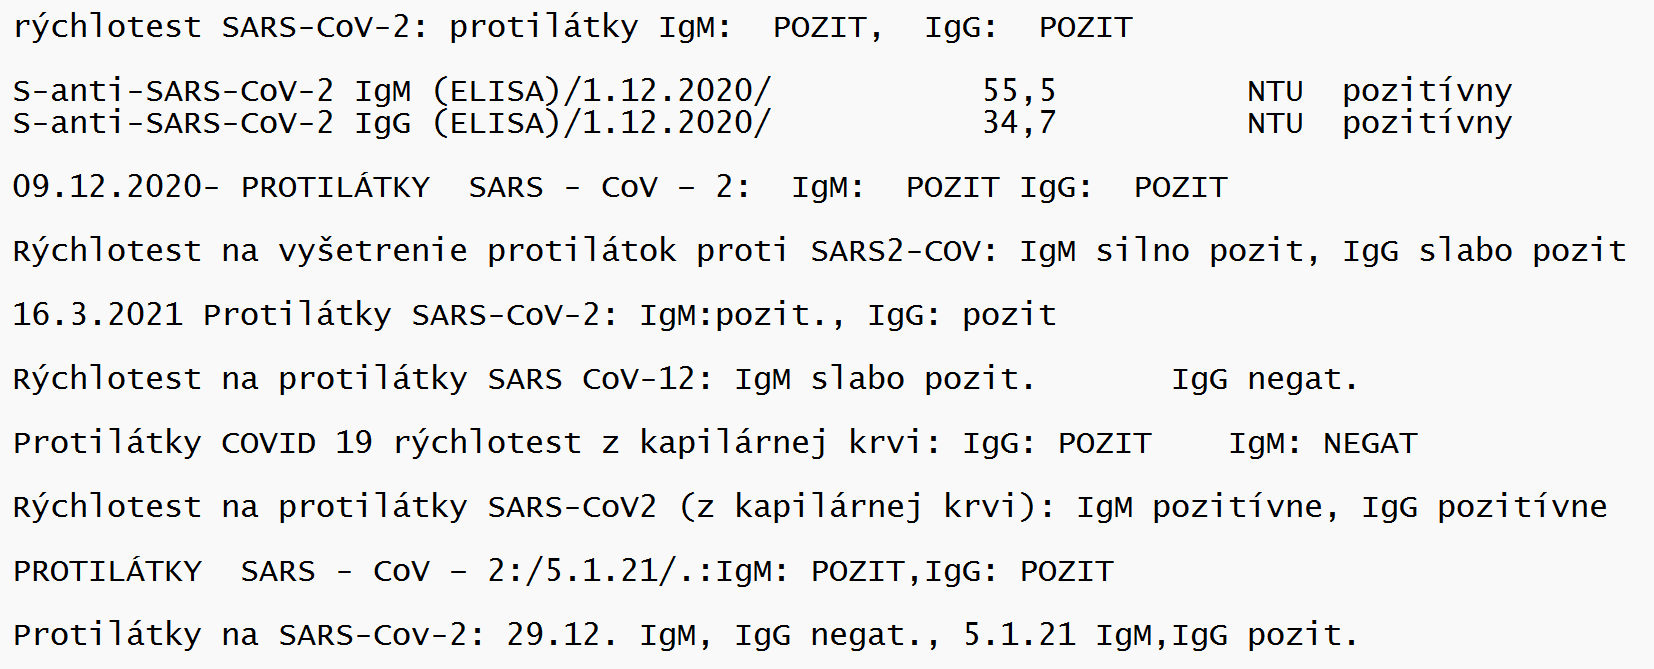
\includegraphics[width=1\textwidth]{images/protilatky}}
	%popis obrazku
	\caption[Protilátky]{Rôzne spôsoby zápisu testov na protilátky v prepúšťacích správach}
	%id obrazku, pomocou ktoreho sa budeme na obrazok odvolavat
	\label{obr:proti}
\end{figure}

Pri hľadaní a následnom získavaní informácie sme využili fakt, že všetky spôsoby zápisu týchto testov obsahujú rovnaké respektíve podobné kľúčové slová a pre nás dôležitú informáciu v rovnakom poradí konkrétne vždy prvým kľúčovým slovom je názov vírusu alebo názov choroby v našom prípade je to vírus SARS-CoV-2 respektíve v niektorých prípadoch ochorenie COVID-19, následne ide kombinácia typov protilátok a samotných výsledkov testov 
 